\documentclass[10pt,spanish,a4paper,openany,notitlepage]{article}
%-------------------------------------Paquetes-----------------------------------------------------------------------
\usepackage[spanish,es-tabla]{babel}  	% Traduce los textos a castellano
\usepackage[utf8]{inputenc}	% Permite escribir directamente áéíóúñ
\usepackage{t1enc}            	% Agrega caracteres extendidos al font
\usepackage{amsmath} 		%Permite imprimir mas opcciones matematicas
\usepackage{graphicx}		%Permite agregar imagenes al informe
\usepackage{multicol}  		%Permite dividir el texto en varias columnas
\usepackage{float} 		%Permite utilizar H para colocar las imagenes en un lugar especifico 
\usepackage{units}
\usepackage{circuitikz}
\usepackage{caption}
\usepackage{subcaption}
\usepackage{sidecap}
\usepackage{mathtools}
\usepackage{multirow} % Paquete para dividir las tablas en subtablas
\usepackage{booktabs} %estos 2 sirven para achicar la tabla
\usepackage{tabulary}
\usepackage{fancyhdr} % encabezado
\usepackage{textcomp} % para usar ° con el comando \textdegree
\usepackage{anysize}		%Permite modificar los margenes del documento
\usepackage{abstract} % paquete para el resumen del articulo
\usepackage{amssymb}
%---------------------------------------Configuraciones de pagina----------------------------------------------
\marginsize{2.5cm}{2.5cm}{1cm}{1cm}

\pagestyle{fancy}
\fancyhf{}
\lhead{
66.25 - \textsc{Dispositivos Semiconductores}\\ 
2\textsuperscript{do} Cuatrimestre de 2014
}
\rhead{
\includegraphics[width=3cm]{imagenes/FIUBA_ALTA.jpg}}
\rfoot{Página \thepage}

%---------------------------------------Definiciones propias---------------------------------------------------------
\newcommand{\oiint}{\displaystyle\bigcirc\!\!\!\!\!\!\!\!\int\!\!\!\!\!\int} %Integral doble cerrada

\DeclarePairedDelimiter\abs{\lvert}{\rvert}%
\DeclarePairedDelimiter\norm{\lVert}{\rVert}%
% Swap the definition of \abs* and \norm*, so that \abs
% and \norm resizes the size of the brackets, and the 
% starred version does not.
\makeatletter
\let\oldabs\abs
\def\abs{\@ifstar{\oldabs}{\oldabs*}}
%
\let\oldnorm\norm
\def\norm{\@ifstar{\oldnorm}{\oldnorm*}}
\makeatother
%--------------------------------------------------------------------------------------------------------------------------------


\makeatletter
\let\ps@plain\ps@fancy 
\makeatother

% lo siguiente es para borrar el titulo del resumen y que no ocupe espacio:
 \AtBeginDocument{%
 \renewcommand{\abstractname}{}%
 }
\renewcommand{\absnamepos}{empty} % originally center
 

\begin{document}
\title{\textbf{TP N\textdegree4: Diseño y construcción de un mini-amplificador de audio}}
\author{
  Accifonte, Franco - 93799\\
  \texttt{franco.accifonte@gmail.com}  
  \and
  Iturria, Germán  - 86270 \\
  \texttt{german.iturria@gmail.com}
  \and
   Vázquez, Matías - 91523\\
  \texttt{mfvazquez@gmail.com}
}
\date{2 de diciembre de 2014}
\maketitle

\begin{abstract} %Resumen
\emph{En el siguiente trabajo se realizará el diseño y construcción de un
mini-amplificador de audio empleando un amplificador de source común. Se
iniciará el diseño mediante cálculos teóricos para luego verificar los
resultados obtenidos mediante simulaciones y finalmente implementar
el circuito. Finalmente se realizarán comparaciones entre los resultados
obtenidos por cada método.}
\end{abstract}

\section{Especificaciones}

Se requiere construir un circuito simple que amplifique la tensión que
genera un micrófono de bobina móvil de $600\, \unit{\Omega}$, considerando
que mantenga una señal de $25\, \unit{m\widehat{V}}$, para que pueda ser digitalizada
por un conversor digital {\bf MAX1393}. El grabador se alimenta con
una batería de $1.5\,\unit{V}$ ($1200\, \unit{mAh}$ de carga), y debe
minimizarse tanto como sea posible el consumo de potencia del sistema.
Las condiciones de diseño del amplificador son:

\begin{itemize}
\item La salida del amplificador debe permitir la máxima excursión
posible entre $0\, \unit{V}$ y $5\, \unit{V}$, que es el rango de entrada
del conversor A/D.
\item La resistencia de salida del amplificador debe ser menor a $5\, \unit{k\Omega}$.
\item La potencia de continua debe ser tal que permita su uso por más de
$24\, \unit{hs}$.
\item Se debe obtener la mayor ganancia posible, respetando lo anterior.
\item El amplificador debe ser emisor común, es decir, debe utilizarse
el transistor {\bf TBJ BC548}.
\item Se debe considerar que la resistencia que presenta el conversor A/D
al amplificador es mayor a $1\, \unit{M\Omega}$.
\end{itemize} 

\section{Diseño del amplificador}

Se definió el circuito mostrado en la figura \ref{circuito:amplificador}.
Utilizando los siguientes valores.
\begin{itemize}
\item $R_S = 600\, \unit{\Omega}$
\item $R_L = 1\, \unit{M\Omega}$
\item $V_{CC} = 1.5\, \unit{V}$
\item $v_s = 25\, \unit{m\widehat{V}}$ 
\item $C_{in} = C_{out} = 1\, \unit{\mu F}$
\end{itemize}

\begin{figure}[H]
\centering
\begin{circuitikz}[american]\shorthandoff{>}
\draw 
(5,1) node[npn](npn){BC548B}
(0,0)  node[ground]{} to [sV, l=$v_s$] (0,1) 
to [R, l=$R_S$] (2,1)
to [C, l=$C_{in}$] (3,1)-- (npn.base)
(2,3) node[ground]{} to [V, l=$V_{CC}$] (2,4)
to [short] (5,4)
to [R, l=$R_C$] (5,2) -- (npn.collector)
(3.5,4) to [R, l=$R_B$] (3.5,1)
(5,0)node[ground]{} -- (npn.emitter) 
(8,0)  node[ground]{} to [R, l_=$R_L$] (8,1.77) 
to [C, l_=$C_{out}$] (5.5,1.77) -- (npn.collector)
;\end{circuitikz}
\caption{Circuito amplificador}
\label{circuito:amplificador}
\end{figure}

Para los cálculos se utilizaron los parámetros obtenidos del transistor 1
en el Trabajo Práctico N\textdegree2 ya que es el transistor que se utilizará
al armar el circuito.

\begin{itemize}
\item $\beta = 361$
\item $V_{th} = 26.95\, \unit{mV}$
\item $V_{A} = 36.05\, \unit{V}$
\item $V_{BE} = 0.7 \, \unit{V}$
\end{itemize}

\subsection{Punto de polarización}

Considerando a los capacitores como circuitos abiertos y 
pasivando la fuente de señal $v_s$ obtenemos el circuito mostrado en 
la figura \ref{circuito:amplificador_dc}.

\begin{figure}[H]
\centering
\begin{circuitikz}[american]\shorthandoff{>}
\draw 
(5,1) node[npn](npn){BC548B}
(2,0) node[ground]{} to [V, l=$V_{CC}$] (2,1)
to [R, l=$R_B$] (4.5,1) --  (npn.base)
(2,1) to [short] (2,2.5)
to [R, l=$R_C$] (5,2.5) -- (npn.collector)
(5,0)node[ground]{} -- (npn.emitter)
(5,2.5) to [short, -o, l=$V_{OUT}$] (5.5,2.5) 
;\end{circuitikz}
\caption{Circuito amplificador en DC}
\label{circuito:amplificador_dc}
\end{figure}

Se consideró la ecuación \ref{eq:VOUT} para los cálculos ya que es
cuando se obtiene la máxima eficiencia.

\begin{equation}
V_{OUT} = \frac{V_{CC}}{2}
\label{eq:VOUT}
\end{equation}

Asumiendo que el TBJ está en MAD y aplicando mallas al circuito de 
la figura \ref{circuito:amplificador_dc} obtenemos las siguientes 
ecuaciones:

\[ \displaystyle V_{CC} - V_{BE} = I_B R_B\]

\[ \displaystyle V_{CC} - V_{OUT} = I_C R_C\]

Y teniendo cuenta que $I_C = \beta I_B$ y la ecuación número \ref{eq:VOUT}
obtenemos las siguientes relaciones de $R_C$ y $R_B$ respecto a $I_C$:

\begin{equation}
R_C = \frac{V_{CC}}{2 I_C}
\label{eq:RC}
\end{equation}

\begin{equation}
R_B = \frac{(V_{CC} - V_{BE}) \beta}{I_C}
\label{eq:RB}
\end{equation}

Luego se verificó que el punto Q este en zona de MAD teniendo en cuenta
la ecuación \ref{eq:RC}:

\[ \displaystyle V_{CE} = V_{CC} - I_C R_C = V_{CC} - \frac{V_{CC}}{2} = \frac{V_{CC}}{2} = 0.75\, \unit{V} > V_{CE_{sat}} \approx 0.2\, \unit{V} \]

Finalmente, debido a que la potencia de continua debe ser tal que permita su uso
por más de $24\, \unit{hs}$ y la batería cuenta con $1200\, \unit{mAh}$
de carga, podemos obtener la cota máxima de la corriente $I_{C}$.
Se consideró también la corriente $I_B$ despreciable respecto a $I_C$,
así toda la corriente suministra la batería será $I_C$.

\[ \displaystyle I_{C} \leqslant \frac{1200\, \unit{mAh}}{24\, \unit{hs}} \]

Por lo tanto:

\begin{equation}
I_{C} \leqslant 50\, \unit{mA}
\label{eq:IC_max}
\end{equation}


\subsection{Modelo de pequeña señal}

Pasivando las fuentes de tensión continua y reemplazando el transistor
por su modelo equivalente de pequeña señal, se obtuvo el circuito
de la figura \ref{circuito:amplificador_ac}.

\begin{figure}[H]
\centering
\begin{circuitikz}[american]\shorthandoff{>}
\draw 
(5,0)  node[ground]{}
(4,0) to [R, l=$R_B$] (4,2) 
(2,2) to [R, l_=$r_{\pi}$, v^=$v_{be}$] (2,0)
(0,0) to [sV, l=$v_s$] (0,2)
to [R,l=$R_S$] (2,2)
to [short] (4,2)
(0,0) to [short] (10,0)
(6,2) to [I,l_=$g_m v_{be}$] (6,0)
(8,0) to [R,l=$r_o$] (8,2)
(10,0) to [R,l=$R_C$] (10,2)
(6,2) to [short] (10,2)
to [short, -o, l=$v_{out}$] (10.5,2)
;\end{circuitikz}
\caption{Circuito amplificador en AC}
\label{circuito:amplificador_ac}
\end{figure}

\begin{equation}
r_\pi = \frac{V_{th} \beta}{I_C}
\label{eq:rpi}
\end{equation}

\begin{equation}
g_m = \frac{I_C}{V_{th}}
\label{eq:gm}
\end{equation}

\begin{equation}
r_o = \frac{V_A}{I_C}
\label{eq:ro}
\end{equation}

Del circuito \ref{circuito:amplificador_ac} se obtiene $v_{out}$

\[ \displaystyle v_{out} = -g_m v_{be} (r_o // R_C) \]

Luego la ganancia de tensión sin carga es

\[ \displaystyle A_{vo} = \frac{v_{out}}{v_{be}} = -gm (r_o // R_C) \]

Reemplazando las ecuaciones \ref{eq:RC}, \ref{eq:gm} y \ref{eq:ro} se obtiene

\[ \displaystyle A_{vo} = -\frac{I_C}{V_{th}} \frac{\frac{V_A V_{CC}}{2 I_C^2}}{\frac{V_A}{I_C} + \frac{V_{CC}}{2 I_C}} \]

Simplificando se obtiene

\begin{equation}
\displaystyle A_{vo} = -\frac{V_A V_{CC}}{V_{th} (2 V_A + V_{CC})}
\label{eq:Avo}
\end{equation}

Es importante notar que $A_{vo}$ sólo depende de $V_{CC}$, ya que
para un mismo transistor $V_A$ y $V_{th}$ permanecen constantes.

Reemplazando los valores obtenemos la ganancia $A_{vo}$

\[ \displaystyle A_{vo} = -28.26 \]

A continuación se analizaron las tres causas de distorsión para obtener las
cotas de $I_C$

\subsubsection{Distorsión por alinealidad}

Para que se pueda utilizar el modelo de pequeña señal del TBJ, se
debe cumplir que $v_{be} \leqslant 10\,\unit{m\widehat{V}}$, ya que este valor es una 
cota máxima en la que una vez superado se pierde la linealidad de las 
ecuaciones utilizadas y se observa la distorsión en la salida con 
respecto a la señal de entrada, por lo tanto se calcula el valor  
máximo de $r_{\pi}$ para que al conectar el micrófono en la entrada 
(con su resistencia interna), la caída de tensión $v_{be}$ no supere este valor 
máximo.

Primero se obtiene la cota de $v_{out}$ para poder compararla con las
cotas de las otras distorsiones. Y recordando que $v_{be}$ y $v_{out}$
están en contra fase:

\[ \displaystyle v_{be;max} = \frac{v_{out;min}}{A_{vo}} = 10\,\unit{m\widehat{V}}\]

Se despeja y calcula $v_{out;min}$

\[ \displaystyle v_{out;min} = v_{be;max} A_{vo} = 10\,\unit{m\widehat{V}} (-28.26) = -282.6 \,\unit{m\widehat{V}}\]

Como $v_{out}$ es una señal sinusoidal $v_{out;max} = -v_{out;min}$ entonces
$v_{out;max} = 282.6 \,\unit{m\widehat{V}}$. 
Por lo tanto la cota de $v_{out}$ para la distorsión por alinealidad será:

\begin{equation}
v_{out} \leqslant 282.6\, \unit{mV}
\label{eq:vout_alinealidad}
\end{equation}


Luego asumiendo que $r_\pi << R_B$ se obtiene $(r_\pi // R_B) \approx r_\pi$.
Con la aproximación anterior resolvemos el divisor de tensión del circuito
de la figura \ref{circuito:amplificador_ac} entre las resistencias $r_\pi$
y $R_S$.

\[ \displaystyle v_{be} = v_s \frac{r_\pi}{R_S + r_\pi} \]

Como $v_{be} \leqslant 10\, \unit{m\widehat{V}}$:

\[ \displaystyle v_s \frac{r_\pi}{R_S + r_\pi} \leqslant 10\,\unit{m\widehat{V}}\]

Despejando $r_\pi$ y reemplazando datos se obtiene:

\begin{equation}
r_\pi \leqslant 400\, \unit{\Omega}
\label{eq:rpi_cota}
\end{equation}

Finalmente reemplazando la ecuación \ref{eq:rpi} en la inecuación \ref{eq:rpi_cota}
se obtiene:

\[ \displaystyle \frac{V_{th} \beta}{I_C} \leqslant 400\, \unit{\Omega} \]

Despejando $I_C$ y reemplazando datos obtenemos:

\begin{equation}
I_C \geqslant 24.32\, \unit{mA}
\label{eq:IC_alinealidad}
\end{equation}

\subsubsection{Distorsión por corte}

Para $v_s$ demasiado negativa el transistor entra en corte, entonces
toda la corriente de señal circula por la resistencia $R_C$.

Se calcula la cota máxima de $v_{out}$, reemplazando la ecuación \ref{eq:VOUT}

\[ \displaystyle v_{out;max} = V_{CC} - V_{OUT} = 1.5\, \unit{V} - 0.75\, \unit{V} = 0.75\, \unit{V} \]

Por lo tanto la cota de $v_{out}$ para la distorsión por corte será:

\begin{equation}
v_{out} \leqslant 750\, \unit{mV}
\label{eq:vout_corte}
\end{equation}

La cota máxima de $v_{out}$ por alinealidad es menor a la cota por corte. Por
lo que evitando la distorsión por alinealidad se estará evitando la
distorsión por corte.

\subsubsection{Distorsión por saturación}

Para $v_s$ muy positiva el TBJ entra en régimen de saturación. El caso
límite tolerable es:

\[ \displaystyle v_{out;max} = V_{OUT} - V_{sat} = 0.75\, \unit{V} - 0.3\, \unit{V} = 0.45\, \unit{V} \]

Por lo tanto la cota de $v_{out}$ para la distorsión por saturación será:

\begin{equation}
v_{out} \leqslant 450\, \unit{mV}
\label{eq:vout_corte}
\end{equation}

Nuevamente la cota máxima de $v_{out}$ por alinealidad es menor a la cota por saturación.
Por lo tanto evitando distorsión por alinealidad se estará también evitando
distorsión por saturación.

\subsection{Elección de $I_C$, $R_C$ y $R_B$}

La cota mínima de $I_C$ es debido a la distorsión por alinealidad y
su cota máxima es debido a que el amplificador pueda ser usado por más
de $24 \unit{hs}$.

\begin{equation}
24.32\, \unit{mA}\leqslant I_C \leqslant 50\, \unit{mA}
\label{eq:IC_cotas}
\end{equation}

Mediante las ecuaciones \ref{eq:RC} y \ref{eq:RB} obtenemos las cotas para $R_C$
y $R_B$, respectivamente.

\begin{equation}
30.84\, \unit{\Omega}\leqslant R_C \leqslant 15\, \unit{\Omega}
\label{eq:RC_cotas}
\end{equation}

\begin{equation}
11.88\, \unit{k\Omega}\leqslant R_B \leqslant 5.78\, \unit{k\Omega}
\label{eq:RB_cotas}
\end{equation}

Finalmente se fijó $I_C = 35\, \unit{mA}$ y en base a ese valor
y a las ecuaciones \ref{eq:RC} y \ref{eq:RB} se calculó $R_C = 21.4\, \unit{\Omega}$ y $R_B = 8.25\, \unit{k\Omega}$.
Como se utilizarán valores normalizados de resistencias se optó por
utilizar $R_C = 25\, \unit{\Omega}$. Para $R_B$ se tomó el valor
normalizado mas cercano al calculado $R_B = 8.2\, \unit{k\Omega}$.

Por lo tanto los valores a utilizar serán:

\[ \displaystyle I_C = 35\, \unit{mA} \]
\[ \displaystyle R_C = 24\, \unit{\Omega}\]
\[ \displaystyle R_B = 8.2\, \unit{k\Omega}\]


\subsection{Cálculo teórico}

Con las $I_C$, $R_C$ y $R_B$ definidas, se realizaron los siguientes
cálculos\footnote{Las tensiones de alterna calculadas serán sus valores
picos positivos, por lo que nos manejaremos con los módulos de las ganancias}:

\begin{itemize}

\item $\displaystyle I_C = 35\, \unit{mA}$

\item $\displaystyle I_B = \frac{I_C}{\beta} = \frac{35\, \unit{mA}}{361} = 96.95\, \unit{\mu A}$

\item $\displaystyle r_\pi = \frac{V_{th}}{I_B} = \frac{26.25\, \unit{mV}}{96.95\, \unit{\mu A}} = 270.76\, \unit{\Omega}$

\item $\displaystyle g_m = \frac{I_C}{V_{th}} = \frac{35\, \unit{mA}}{26.25\, \unit{mV}} = 1.34\, \unit{\frac{A}{V}}$

\item $\displaystyle r_o = \frac{V_A}{I_C} = \frac{36.05\, \unit{V}}{35\, \unit{mA}} = 1.03\, \unit{k\Omega}$

\item $\displaystyle v_{in} = v_{be} = v_s \frac{r_\pi}{R_S + r_\pi} = 25\,\unit{m\widehat{V}} \frac{270.76\, \unit{\Omega}}{600 \unit{\Omega} + 270.76\, \unit{\Omega}} = 7.78\,\unit{m\widehat{V}}$

\item $\displaystyle \abs{A_{vo}} = 28.26$

\item $\displaystyle v_{out} = \abs{A_{vo}} v_{in} = 28.26\  7.78\,\unit{m\widehat{V}} = 219.86\,\unit{m\widehat{V}}$

\item $\displaystyle \abs{A_{vs}} = \frac{v_{out}}{v_s} = \frac{219.86\,\unit{m\widehat{V}}}{25\,\unit{m\widehat{V}}} = 8.79$

\item $\displaystyle V_{BE} = V_{CC} - I_B R_B = 1.5\, \unit{V} - 96.95\, \unit{\mu A}\ 10\, \unit{k\Omega} = 530.5\, \unit{mV}$

\item $\displaystyle V_{CE} = V_{CC} - I_C R_C = 1.5\, \unit{V} - 35\, \unit{mA}\ 24\, \unit{\Omega} = 660\, \unit{mV}$

\item $\displaystyle R_{IN} = r_\pi//R_B = \frac{270.76\, \unit{\Omega}\ 8.2\, \unit{k\Omega}}{270.76\, \unit{\Omega} + 8.2\, \unit{k\Omega}} = 262.1\, \unit{\Omega}$

\item $\displaystyle R_{OUT} = r_o // R_C = \frac{1.03\, \unit{k\Omega}\ 25\, \unit{\Omega}}{1.03\, \unit{k\Omega} + 25\, \unit{\Omega}} = 24.41\, \unit{\Omega}$

\item $\displaystyle \eta = \frac{P_{OUT}}{P_{DC}} = \frac{\frac{v_{out}^2}{2 R_C}}{V_{CC} I_C} = \frac{v_{OUT}^2}{2 R_C V_{CC} I_C} = \frac{(625\,\unit{mV})^2}{2\ 24\, \unit{\Omega}\ 1.5\, \unit{V}\ 35\, \unit{mA}} = 0.155 \Longrightarrow \eta_{\%} = 15.5\, \unit{\%} $


\end{itemize}

\subsection{Dispersión de $\beta$}

De la hoja de datos se obtuvieron $\beta_{min} = 200$ y $\beta_{max} = 450$
En la ecuación \ref{eq:Avo} se deduce que $A_{vo}$ solo depende de $V_{CC}$
por lo tanto la variación de $\beta$ no afectará a la ganancia.

Al cambiar $\beta$ la tensión $V_{BE}$ será constante dado que es el terminal
de control. La tensión $V_{CE}$ variará debido a que $I_C$ variará y por
ende variará la tensión en $R_C$.

Se calculó $I_C$ y $V_{CE}$ para los distintos $\beta$ siendo:
\[ \displaystyle I_B =  96.95\, \unit{\mu A}\]
\[ \displaystyle V_{BE} =  530.5\, \unit{mV}\]
\[ \displaystyle \abs{A_{vo}} = 28.26 \] 

para ambos casos ya que no varían.



\begin{itemize}

\item $\beta = \beta_{min} = 200$

	\begin{itemize}
	\item $\displaystyle I_C = I_B \beta = 96.95\, \unit{\mu A}\ 200 = 19.39\, \unit{mA}$
	\item $\displaystyle V_{CE} = V_{CC} - I_C R_C = 1.5\, \unit{V}\ - 19.39\, \unit{mA}\ 24\, \unit{\Omega} = 1.03\, \unit{V}$
	\end{itemize}

\item $\beta = \beta_{max} = 450$

	\begin{itemize}
	\item $\displaystyle I_C = I_B \beta = 96.95\, \unit{\mu A}\ 450 = 43.63\, \unit{mA}$
	\item $\displaystyle V_{CE} = V_{CC} - I_C R_C = 1.5\, \unit{V}\ - 43.63\, \unit{mA}\ 24\, \unit{\Omega} = 453\, \unit{mV}$
	\end{itemize}

\end{itemize}

Cuando $\beta = \beta_{min} = 200$ el valor de $I_C$ esta por debajo
de la cota mínima de la inecuación \ref{eq:IC_cotas}.
Por lo tanto la señal de salida estará distorsionada por alinealidad y
por esta razón no es un diseño robusto ya que la variación de $\beta$
es muy amplia.


\subsection{Comparación con source común}

Comparando las configuraciones Source común y Emisor común, se observa 
que la configuración source común posee una alta impedancia de entrada(infinita), 
mientras que la configuración Emisor común posee una mediana impedancia de 
entrada $r_\pi//R_B$.  Con respecto  a la impedancia de salida, las dos 
configuraciones poseen un rango medio, en Source común su valor es $r_o//R_D$  y en Emisor común 
vale $r_o//R_C$.  Dado que sus valores de ro resultan similares, 
se puede decir que poseen una impedancia de salida parecida.

Una ventaja del uso de transistores MOSFET es que se lograría evitar
la dispersión de $\beta$. 

\section{Simulación del circuito}

Se simuló mediante \emph{Spice} el circuito de la figura \ref{circuito:amplificador}.
Siendo $R_C = 24\, \unit{\Omega}$ y $R_B = 8.2\, \unit{k\Omega}$ y
los capacitores de $1\, \unit{\mu F}$.
Se utilizó como transistor un modelo genérico modificado con los datos
del transistor utilizado en los cálculos teóricos. Utilizamos este modelo
de transistor ya que es el que tiene menos diferencias con el transistor
que se utilizará, especialmente por tener el mismo $\beta$. Para agregarle los
parámetros se aplicó el siguiente comando:\\

\texttt{.MODEL MiModelo NPN (BF=361 IS=106.239f VAF=36.05432)}\\

Luego se obtuvieron todos los parámetros calculados en la sección anterior:

\begin{itemize}

\item $\displaystyle I_C = 36\, \unit{mA}$

\item $\displaystyle I_B = 100\, \unit{\mu A}$

\item $\displaystyle r_\pi = \frac{V_{th}}{I_B} = \frac{26.25\, \unit{mV}}{100\, \unit{\mu A}} = 262.5\, \unit{\Omega}$

\item $\displaystyle g_m = \frac{I_C}{V_{th}} = \frac{36\, \unit{mA}}{26.25\, \unit{mV}} = 1.37\, \unit{\frac{A}{V}}$

\item $\displaystyle r_o = \frac{V_A}{I_C} = \frac{36.05\, \unit{V}}{36\, \unit{mA}} = 1\, \unit{k\Omega}$

\item $\displaystyle v_{in} = v_{be} = 7.5\,\unit{m\widehat{V}}$

\item $\displaystyle v_{out} = 250\,\unit{m\widehat{V}}$

\item $\displaystyle \abs{A_{vo}} =  \frac{v_{out}}{v_{in}} = \frac{250\,\unit{m\widehat{V}}}{7.5\,\unit{m\widehat{V}}} = 33.34$

\item $\displaystyle \abs{A_{vs}} = \frac{v_{out}}{v_s} = \frac{250\,\unit{m\widehat{V}}}{25\,\unit{m\widehat{V}}} = 10$

\item $\displaystyle V_{BE} = 685.5\, \unit{mV}$

\item $\displaystyle V_{CE} = 600\, \unit{mV}$

\item $\displaystyle \eta = \frac{v_{OUT}^2}{2 R_C V_{CC} I_C} = \frac{(600\,\unit{mV})^2}{2\ 24\, \unit{\Omega}\ 1.5\, \unit{V}\ 36\, \unit{mA}} = 0.1389 \Longrightarrow \eta_{\%} = 13.89\, \unit{\%} $

\end{itemize}

\subsection{Obtención de $R_{IN}$}

Simulamos un circuito equivalente al mostrado en la figura 
\ref{circuito:simulacion_RIN} siendo el esquema amplificador el 
amplificador diseñado. Utilizamos una fuente de prueba $v_p$ con un valor
de forma que el amplificador no distorsione. Y una resistencia $R_p \approx R_{IN}$
utilizando como referencia el $R_{IN} = 262.1\, \unit{\Omega}$ obtenido
en los cálculos teóricos. Por lo tanto los datos utilizados en el circuito
fueron:

\[ \displaystyle v_p = 10\, \unit{m\widehat{V}}\]
\[ \displaystyle R_p = 262.1\, \unit{\Omega}\]
\[ \displaystyle C_{in} = C_{out} = 1\, \unit{\mu F}\]

\begin{figure}[H]
\centering
\begin{circuitikz}[american]\shorthandoff{>}
\draw
(0,0) to [sV, l=$v_p$] (0,2)
to [R, l=$R_p$] (2,2)
to [C, l=$C_{in}$] (4,2)
to [short] (5,2)
to [R, l_=$R_{IN}$] (5,0)
to [short] (0,0)
(2.25,2) to [open, o-o, v=$v_x$] (2.25,0)

(12,0) to [short, o-] (7,0)
to [sV, l=$A_{vo}v_i$] (7,2)
to [R, l=$R_{OUT}$] (10,2)
to [C, l=$C_{out}$, -o] (12,2)

(3.5,-1) to [short] (3.5,3)
to [short] (9.5,3)
to [short] (9.5,-1)
to [short, l= esquema amplificador](3.5,-1)

;\end{circuitikz}
\caption{Circuito para la obtención de $R_{IN}$}
\label{circuito:simulacion_RIN}
\end{figure}

Se obtuvo de la simulación la tensión $v_x = 5.5\, \unit{m\widehat{V}}$.
Luego se planteó el divisór de tensión entre $R_p$ y $R_{IN}$ despreciando
la impedancia del capacitor $Z_C$ frente a las resistencias:

\[ \displaystyle v_x = v_p \frac{R_{IN}}{R_p + R_{IN}} \]

Se despejó $R_{IN}$ y se calculó reemplazando los datos:

\[ \displaystyle R_{IN} = R_p \frac{v_x}{v_p - v_x} = 262.1\, \unit{\Omega} \frac{5.5\, \unit{m\widehat{V}}}{10\, \unit{m\widehat{V}} - 5.5\, \unit{m\widehat{V}}} = 320.34 \unit{\Omega}\]

\subsection{Obtención de $R_{OUT}$}

Finalmente para obtener $R_{OUT}$ primero se simuló un circuito equivalente
al mostrado en la figura \ref{circuito:simulacion_Avovi} donde el esquema
amplificador es el amplificador diseñado. Se utilizó una fuente $v_i = 1\, \unit{m\widehat{V}}$
para no obtener distorsión en la señal de salida. Y se obtuvo la tensión
$A_{vo}v_i = 28.2\, \unit{m\widehat{V}}$.


\begin{figure}[H]
\centering
\begin{circuitikz}[american]\shorthandoff{>}
\draw
(1,0) to [sV, l=$v_{i}$] (1,2)
to [C, l=$C_{in}$] (4,2)
to [short] (5,2)
to [R, l_=$R_{IN}$] (5,0)
to [short] (1,0)
(3,2) to [open, o-o,] (3,0)

(12,2) to [open, v=$A_{vo}v_i$, o-o] (12,0)
 to [short] (10,0)
to [short] (7,0)
to [sV, l=$A_{vo}v_i$] (7,2)
to [R, l=$R_{OUT}$] (10,2)
to [C, l=$C_{out}$] (12,2)


(3.5,-1) to [short] (3.5,3)
to [short] (9.5,3)
to [short] (9.5,-1)
to [short,l= esquema amplificador](3.5,-1)

;\end{circuitikz}
\caption{Circuito para la obtención de $A_{vo}v_i$}
\label{circuito:simulacion_Avovi}
\end{figure}

Finalmente se simuló el circuito de la figura \ref{circuito:simulacion_ROUT}
Siendo el amplificador diseñado el esquema amplificador de la figura.
Se utilizó la misma resistencia de salida obtenida en los cálculos teóricos
como resistencia de prueba $R_p = 24.41\, \unit{\Omega}$. Se obtuvo
el valor de $v_o = 4.2\, \unit{m\widehat{V}}$.
Luego se planteó la ecuación del divisor de tensión entre las resistencias
$R_{OUT}$ y $R_p$:

\[ \displaystyle v_o = A_{vo}v_i \frac{R_p}{R_{OUT} + R_p} \]

Despejando y reemplazando los datos se obtuvo $R_{OUT}$:

\[ \displaystyle R_{OUT} = R_p \Bigg(\frac{A_{vo}v_i}{v_o} -1\Bigg) = R_p = 24.41\, \unit{\Omega} \Bigg(\frac{28.2\, \unit{m\widehat{V}}}{4.2\, \unit{m\widehat{V}}} -1\Bigg) = 139.5 \unit{\Omega}\]

\begin{figure}[H]
\centering
\begin{circuitikz}[american]\shorthandoff{>}
\draw
(1,0) to [sV, l=$v_{i}$] (1,2)
to [C, l=$C_{in}$] (4,2)
to [short] (5,2)
to [R, l_=$R_{IN}$] (5,0)
to [short] (1,0)
(3,2) to [open, o-o,] (3,0)

(12,2) to [R, l = $R_p$, v=$v_o$, o-o] (12,0)
 to [short] (10,0)
to [short] (7,0)
to [sV, l=$A_{vo}v_i$] (7,2)
to [R, l=$R_{OUT}$] (10,2)
to [C, l=$C_{out}$] (12,2)


(3.5,-1) to [short] (3.5,3)
to [short] (9.5,3)
to [short] (9.5,-1)
to [short, l= esquema amplificador](3.5,-1)

;\end{circuitikz}
\caption{Circuito para la obtención de $R_{OUT}$}
\label{circuito:simulacion_ROUT}
\end{figure}

\subsection{Señal obtenida}

En la figura \ref{fig:simulacion_entrada_salida} se puede comparar la señal
de entrada y salida simuladas. En donde calculamos la diferencia entre
los módulos del valor máximo y mínimo de $v_{out}$:

\[ \displaystyle  \abs{v_{out;max} + v_{out;min}} = \abs{238.72\, \unit{mV} - 247.72\, \unit{mV}} = 9\, \unit{mV} \]

Que podemos considerar desprececiable respecto a $v_{out;max}$ y $v_{out;min}$.

\begin{figure}[H]
\centering
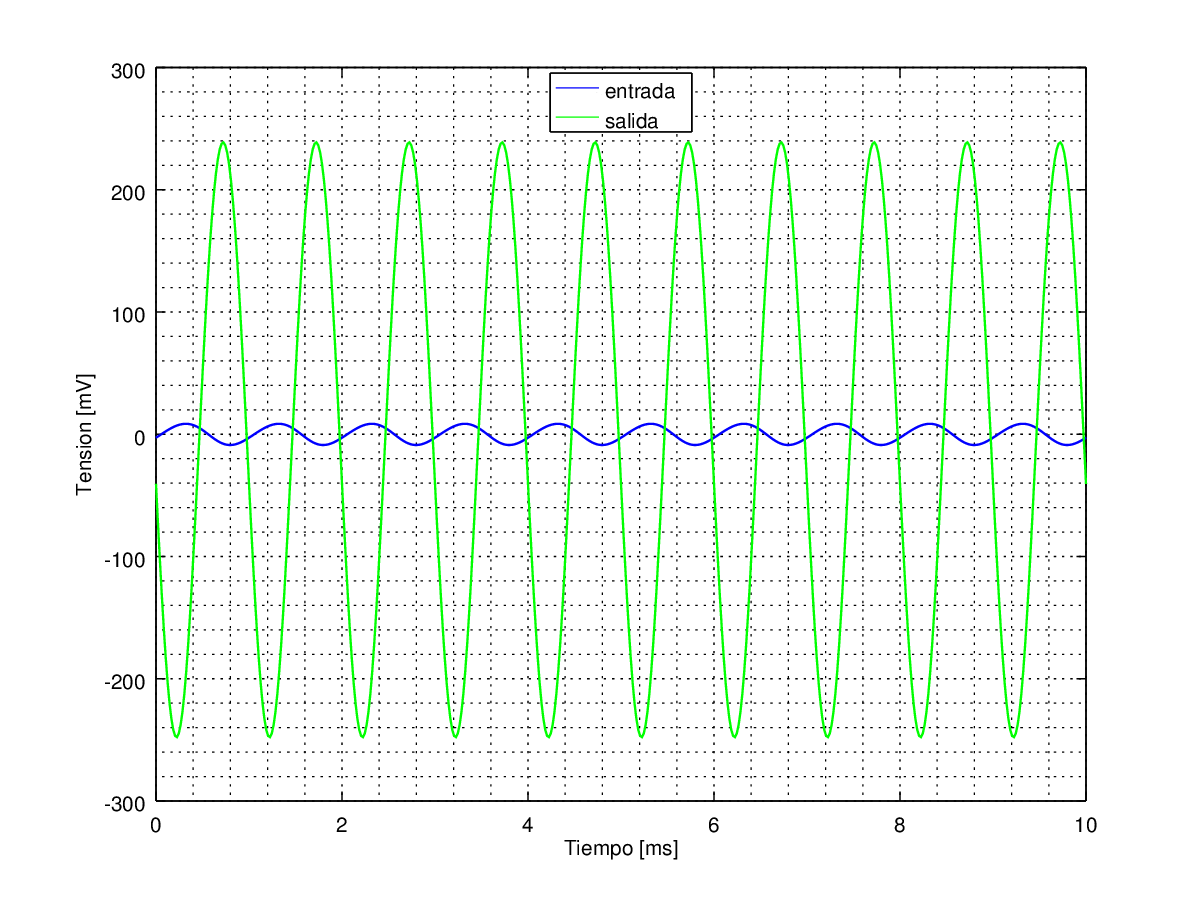
\includegraphics[scale=0.8]{./octave/grafico.png}
\caption{Señales de entrada y salida de la simulación.}
\label{fig:simulacion_entrada_salida}
\end{figure}

\subsection{Comparación de los resultados}

A continuación se comparan las diferencias obtenidas en los parámetros
mediante simulación respecto al cálculo teórico.

\begin{table}[H]
\centering
\begin{tabular}{|c|c|c|c|}
\hline
$X$ & Cálculo teórico & Simulación & $\frac{X_{teorico} - X_{simulación}}{X_{teórico}}\ 100 \unit{\%}$ \\
\hline
$I_C $ & $35\, \unit{mA} $ 		& $36\, \unit{mA} $ & $-2.8\, \unit{\%} $ \\
\hline
$I_B $ & $96.95\, \unit{\mu A} $	 & $100\, \unit{\mu A} $ & $-3.1\, \unit{\%} $ \\
\hline
$r_\pi $ & $270.76\, \unit{\Omega} $	 & $262.5\, \unit{\Omega} $ & $3.1\, \unit{\%} $ \\
\hline
$g_m $ & $1.34\, \unit{A/V} $ 	& $1.37\, \unit{A/V} $ & $-2.2\, \unit{\%} $ \\
\hline
$r_o $ & $1.03\, \unit{k\Omega} $ 	& $1\, \unit{k\Omega} $ & $2.9\, \unit{\%} $ \\
\hline
$v_{in} $ & $7.78\, \unit{m\widehat{V}} $	 & $7.5\, \unit{m\widehat{V}} $ & $3.6\, \unit{\%} $ \\
\hline
$\abs{A_{vo}} $ & $28.26$ 	& $33.34 $ & $-18.0\, \unit{\%} $ \\
\hline
$v_{out} $ & $218.86\, \unit{m\widehat{V}} $ 	& $250\, \unit{m\widehat{V}} $ & $-14.2\, \unit{\%} $ \\
\hline
$\abs{A_{vs}} $ & $8.79$ 	& $10 $ & $-13.8\, \unit{\%} $ \\
\hline
$V_{BE} $ & $530.5\, \unit{mV} $ 	& $685.5\, \unit{mV} $ & $-29.2\, \unit{\%} $ \\
\hline
$V_{CE} $ & $625\, \unit{mV} $ 	& $600\, \unit{mV} $ & $4.0\, \unit{\%} $ \\
\hline
$R_{IN} $ & $262.1\, \unit{\Omega} $ 	& $320.34\, \unit{\Omega} $ & $22.2\, \unit{\%} $ \\
\hline
$R_{OUT} $ & $24.41\, \unit{\Omega} $ 	& $138.5\, \unit{\Omega} $ & $-467.4\, \unit{\%} $ \\
\hline
$\eta_{\%} $ & $14.88\, \unit{\%} $ 	& $13.34\, \unit{\%} $ & $10.3\, \unit{\%} $ \\
\hline
\end{tabular}
\caption{Comparación de valores obtenidos mediante simulación y cálculo teórico}
\label{table:comparacion_simulacion}
\end{table}

\section{Mediciones del circuito}

Se armó en un \emph{protoboard} el circuito del amplificador diseñado
mostrado en la figura \ref{circuito:amplificador}  y re realizaron las mediciones. 
de todos los parámetros antes calculados.
Siendo $R_C = 24\, \unit{\Omega}$ y $R_B = 8.2\, \unit{k\Omega}$ resistencias
con tolerancia del $1\, \unit{\%}$ y
los capacitores de $1\, \unit{\mu F}$.

\subsection{Emulación de la fuente de señal y la carga}

Como no se dispuso de un generador que llegue a $25\, \unit{m\widehat{V}}$
sin distorsión y con resistencia serie de $600\, \unit{\Omega}$. Se emuló
un circuito de micrófono utilizando un generador con resistencia serie de
$R_g = 50\, \unit{\Omega}$.

Se partió del circuito mostrado en la figura \ref{circuito:microfono}.
Fijando $v_g = 100\, \unit{m\widehat{V}}$ y sabiendo que la tensión de
salida $v_x = 25\, \unit{m\widehat{V}}$ se resolvió el divisor de
tensión entre la resistencia interna del generador $R_g$ y $R_1$

\[ \displaystyle v_x = v_g \frac{R_1}{R_1 + R_g} \]

Despejando $R_1$ y reemplazando datos:

\[ \displaystyle R_1 = R_g \frac{v_x}{v_g - v_x} = 50\, \unit{\Omega} \frac{25\, \unit{m\widehat{V}}}{100\, \unit{m\widehat{V}} - 25\, \unit{m\widehat{V}}} = 16.7\, \unit{\Omega} \]

Luego se eligió un valor normalizado para $R_1$ cercano al calculado y
modificamos $v_g$ para obtener la tensión de salida deseada. Por lo tanto
se optó por elegir 
\[ \displaystyle R_1 = 18\, \unit{\Omega}\]

\begin{figure}[H]
\centering
\begin{circuitikz}[american]\shorthandoff{>}
\draw
(4,0) to [short] (0,0)
to [sV, l=$v_g$] (0,2)
to [R, l= $R_g$] (2,2)
to [R, l= $R_1$] (2,0)
(2,2) to [R, l=$R_2$] (4,2)
to [open, o-o, v=$v_x$] (4,0)
;\end{circuitikz}
\caption{Circuito emulador de micrófono}
\label{circuito:microfono}
\end{figure}

Para obtener $R_2$ se pasivó la fuente $v_g$ y se obtuvo $R_2$ de forma tal
que la resistencia equivalente del circuito emulador de micrófono sea de
$600\, \unit{\Omega}$. Tal como se muestra en el circuito de la figura
\ref{circuito:microfono_req}.

Obteniendo las resistencias equivalentes se llega a:

\[ \displaystyle R_{eq} = (R_g // R_1) + R_2 \]

Despejando y reemplazando datos obtenemos $R_2$

\[ \displaystyle R_2 = R_{eq} - (R_g//R_1) = 600\, \unit{\Omega} - \frac{50\, \unit{\Omega}\ 18\, \unit{\Omega}}{50\, \unit{\Omega} + 18\, \unit{\Omega}} =  586.8\, \unit{\Omega}\]

Finalmente se eligió un valor para $R_2$ normalizado cercano al calculado.
Por lo tanto:

\[ \displaystyle R_2 = 620\, \unit{\Omega}\]

\begin{figure}[H]
\centering
\begin{circuitikz}[american]\shorthandoff{>}
\draw
(4,0) to [short] (0,0)
to [short] (0,2)
to [R, l= $R_g$] (2,2)
to [R, l= $R_1$] (2,0)
(2,2) to [R, l=$R_2$] (4,2)
to [open, o-o, v=$v_x$] (4,0)
;\end{circuitikz}
\caption{Circuito emulador de micrófono con fuente pasivada}
\label{circuito:microfono_req}
\end{figure}

Finalmente para verificar que la resistencia interna del circuito emulador de
micrófono sea la deseada, se conectó una resistencia de prueba
$R_x = 620\, \unit{\Omega}$ y se midió con el osciloscopio el valor pico de la tensión
$v_x = 12\, \unit{m\widehat{V}}$ como se muestra en la figura \ref{circuito:medicion_RS}.
Siendo $v_{in} = 25\, \unit{m\widehat{V}}$ se planteó el divisor de tensión
entre $R_S$ y $R_x$:

\[ \displaystyle v_x = v_{in} \frac{R_x}{R_x + R_S} \]

Despejamos $R_S$ y reemplazamos datos:

\[ \displaystyle R_S = R_x \frac{v_{in} - v_x}{v_x} = 620\, \unit{\Omega} \frac{25\, \unit{m\widehat{V} - 12\, \unit{m\widehat{V}}}}{12\, \unit{m\widehat{V}}} = 671.7\, \unit{\Omega} \]

\begin{figure}[H]
\centering
\begin{circuitikz}[american]\shorthandoff{>}
\draw
(2,0) to [short] (0,0)
to [sV, l=$v_{in}$] (0,2)
to [R, l= $R_S$] (2,2)
to [R,l= $R_x$, o-o, v_=$v_x$] (2,0)
;\end{circuitikz}
\caption{Circuito equivalente del micrófono para la medición de $R_S$}
\label{circuito:medicion_RS}
\end{figure}

\subsection{Mediciones del circuito}

Una vez con el circuito armado se realizaron mediciones comparativas
con el osciloscopio midiendo la tensión de entrada y salida. Como
resultado se obtuvieron las señales de la figura \ref{fig:medicion_entrada_salida}.

\begin{figure}[H]
\centering
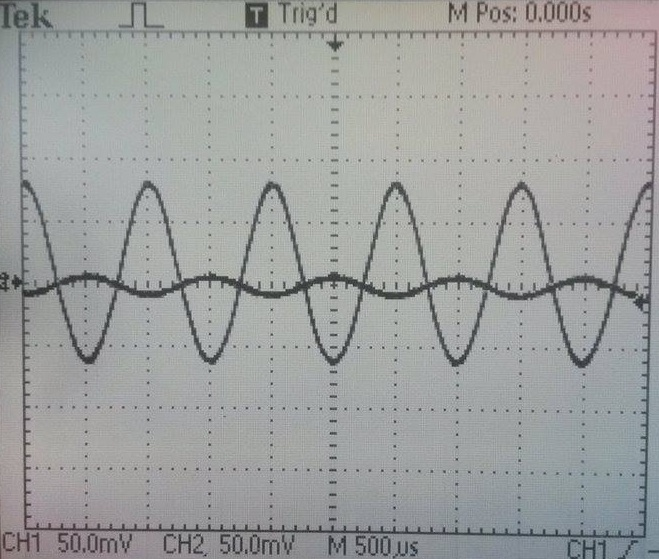
\includegraphics[scale=0.8]{./imagenes/experimental_entrada_salida.jpg}
\caption{Señales de entrada y salida de la medición.}
\label{fig:medicion_entrada_salida}
\end{figure}

Como se puede apreciar la señal de salida se encuentra distorsionada. Alcanza
un valor pico de $75\, \unit{m\widehat{V}}$ cuando en la simulación se
alcanzó un valor de $240\, \unit{m\widehat{V}}$. Esto ocurre debido
al mal funcionamiento del transistor utilizado ya que en las hojas de
datos se indica que con $V_{CE} = 0.3\, \unit{V}$ deberia estar MAD. 
Como podemos ver en la
figura \ref{fig:ic_vce} obtenida en el Trabajo Práctico N\textdegree2
el transistor entra en región de MAD al alcanzar una tensión 
$V_{CE} \approx 1.4\, \unit{V}$ y contando solo con una fuente $V_{CC} = 1.5\, \unit{V}$
no hay manera de obtener una señal sin distorsión ya que no se puede alcanzar
la región de MAD.

\begin{figure}[H]
\centering
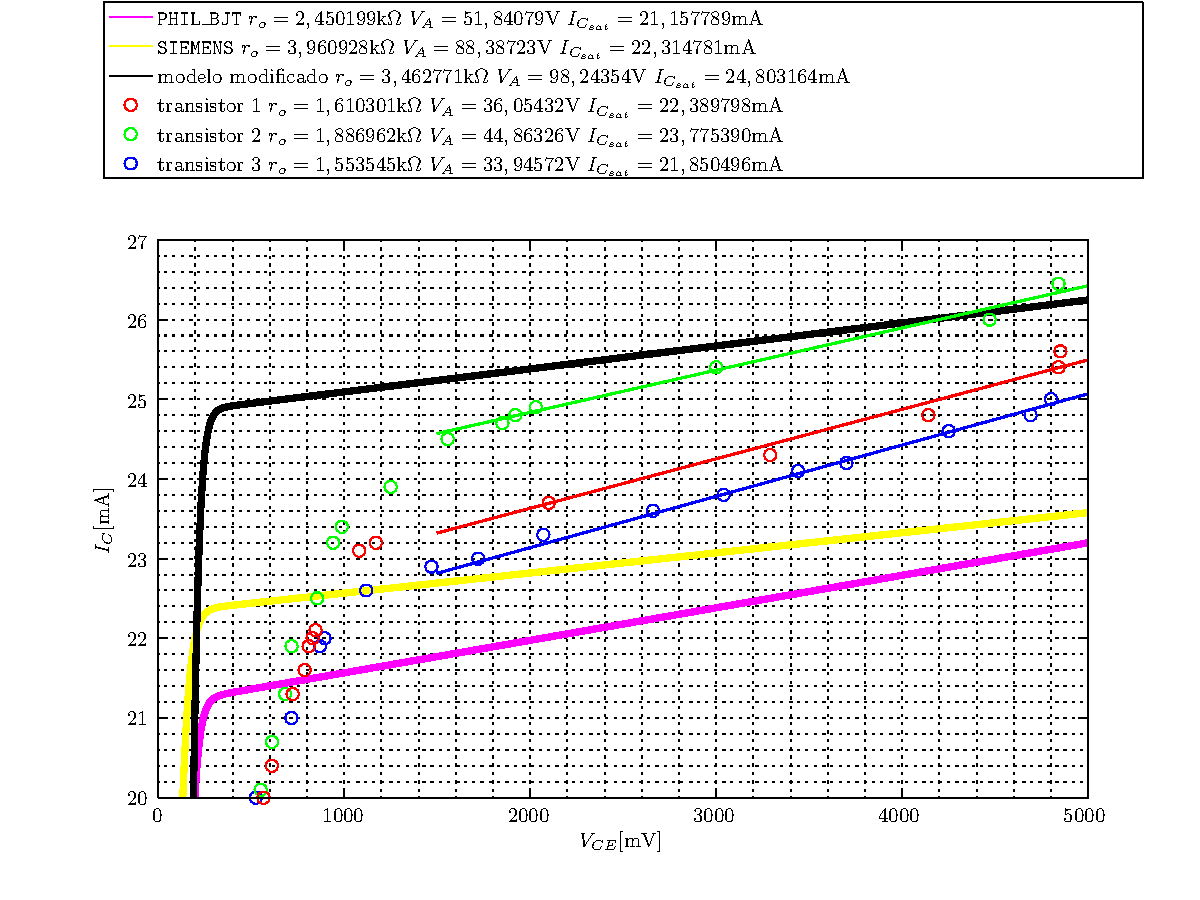
\includegraphics[scale=0.8]{./imagenes/IcvsVce_25mA.pdf}
\caption{Gráfico $I_C$ vs. $V_{CE}$.}
\label{fig:ic_vce}
\end{figure}

\begin{table}[H]
\centering
\begin{tabular}{|c|c|c|c|}
\hline
Parámetro & Transistor 1 & Transistor 2 & Transistor 3 \\
\hline
$\beta$ & $361$ & $253$ & $326$ \\
\hline
$V_{CE}$ & $878\, \unit{mV}$ & $1016\, \unit{mV}$ & $932\, \unit{mV}$ \\
\hline
$V_{BE}$ & $732\, \unit{mV}$ & $724\, \unit{mV}$ & $726\, \unit{mV}$ \\
\hline
$I_C$ & $27.48\, \unit{mA}$ & $21.92\, \unit{mA}$ & $25.24\, \unit{mA}$ \\
\hline
\end{tabular}
\caption{Comparación de valores medidos para distintos transistores}
\label{table:comparacion_medicion}
\end{table}

\section{Conclusiones}

Como principal conclusión se debe remarcar la importancia de verificar
el correcto funcionamiento de los componentes antes de utilizarlos. En
este trabajo se utilizaron transistores con los cuales no se pudo obtener
una señal amplificada sin distorsiones debido a que la tensión $V_{CE}$
para entrar en régimen MAD era mayor a la obtenida en las hojas de datos.
Por eso es importante haber verificado antes las curvas de salida del
transistor.

Otro problema importante es la dispersión del $\beta$ ya que el circuito
diseñado puede presentar distorsiones con distintos transistores. Por
lo que sería necesario utilizar circuitos realimentados para evitar la
dispersión del $\beta$.

Se deben tener en cuenta las posibles distorsiones que pueda presentar
la señal de salida. Ya que son los principales limitantes de los parámetros
que se deben elegir para armar el circuito.



\end{document}
